\setcounter{section}{0}
\section{Lý thuyết}
\subsection{Năng lượng}
\subsubsection{Khái niệm năng lượng}
Năng lượng tồn tại ở khắp mọi nơi xung quanh chúng ta. Mọi hiện tượng xảy ra trong tự nhiên đều cần có năng lượng dưới các dạng khác nhau như: cơ năng, hóa năng, nhiệt năng, điện năng, năng lượng ánh sáng, năng lượng âm thanh, năng lượng nguyên tử.
\subsubsection{Tính chất của năng lượng}
\begin{itemize}
	\item Năng lượng là một đại lượng vô hướng;
	\item Năng lượng không tự sinh ra hoặc tự mất đi mà chỉ chuyển hóa từ dạng này sang dạng khác hoặc truyền từ vật này sang vật khác;
	\item Trong hệ SI, năng lượng có đơn vị là joule (J).\\ Một đơn vị năng lượng khác là calorie. Một calorie là năng lượng cần thiết để làm tăng nhiệt độ $\SI{1}{g}$ nước lên thêm $\SI{1}{\celsius}$.
	$$\SI{1}{cal} = \SI{4.184}{J}$$
\end{itemize}

\subsection{Công cơ học}
%	\begin{center}
	%	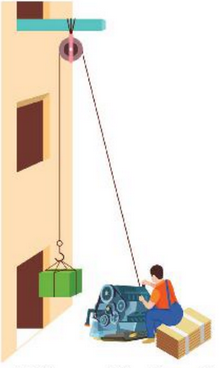
\includegraphics[scale=0.6]{../figs/G10-018-1}
	%\end{center}
	
	\subsubsection{Điều kiện có công cơ học}
	Một lực sinh công khi nó tác dụng lên một vật và điểm đặt của lực chuyển dời.
	
	
	\subsubsection{Khái niệm công cơ học}
	Nếu lực không đổi $\vec{F}$ tác dụng lên một vật và điểm đặt của lực đó chuyển dời một đoạn $s$ theo hướng hợp với hướng của lực góc $\alpha$ thì công của lực $\vec{F}$ được tính theo công thức
	\begin{equation*}
		A=Fs\cos \alpha.
	\end{equation*}
	\begin{center}
		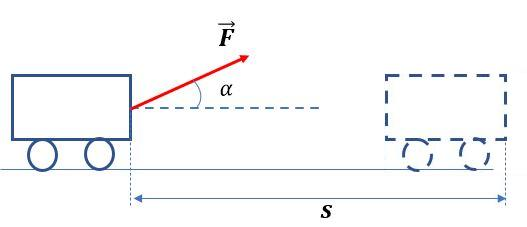
\includegraphics[scale=0.6]{../figs/VN10-PH-30-L-022-1-3.jpg}
	\end{center}
	\subsubsection{Đơn vị của công}
	Trong hệ SI, đơn vị của công là joule (kí hiệu là J).
	
	$$1\ \text{N} \cdot 1\ \text{m}= 1\ \text{J}$$
	
	1 joule là công do lực có độ lớn 1 newton thực hiện khi điểm đặt của lực chuyển dời 1 mét theo hướng của lực.
	\subsubsection{Công phát động, công cản}
	\begin{itemize}
		\item Khi $\alpha$ là góc nhọn thì $\cos \alpha >0$, suy ra $A>0$: $A$ gọi là công phát động.
		\begin{center}
			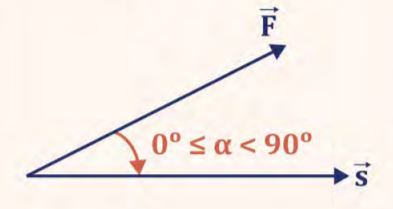
\includegraphics[scale=0.5]{../figs/VN10-PH-30-L-022-1-4.JPG}
		\end{center}
		\item Khi $\alpha = 90^\circ$ thì $\cos 
		\alpha = 0$, suy ra $A=0$: lực $\vec{F}$ không sinh công.
		\item Khi $\alpha$ là góc tù thì $\cos \alpha <0$, suy ra $A<0$: $A$ gọi là công cản.
		\begin{center}
			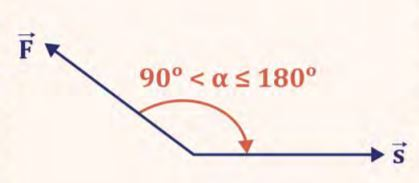
\includegraphics[scale=0.55]{../figs/VN10-PH-30-L-022-1-5.JPG}
		\end{center}
	\end{itemize}
	\luuy{Các công thức tính trên chỉ đúng khi điểm đặt của lực chuyển dời thẳng và lực không đổi trong quá trình chuyển động.}
	
	
	\section{Mục tiêu bài học - Ví dụ minh họa}
	\begin{dang}{Nhắc lại khái niệm năng lượng ở THCS. \\Quá trình chuyển hóa năng lượng}
		\viduii{1}{Kể tên các dạng năng lượng mà em biết.
		}
		{\begin{center}
				\textbf{Hướng dẫn giải}
			\end{center}
			
			Học sinh có thể kể đến những dạng năng lượng như: cơ năng, hóa năng, nhiệt năng, điện năng, năng lượng ánh sáng, năng lượng âm thanh, năng lượng nguyên tử.
		}
		
		\viduii{2}{Một thỏi sô-cô-la có khối lượng $\SI{60}{g}$ chứa $\SI{280}{cal}$ năng lượng. Hãy tính lượng năng lượng của thỏi sô-cô-la này theo đơn vị joule.
		}
		{\begin{center}
				\textbf{Hướng dẫn giải}
			\end{center}
			
			Ta có $\SI{1}{cal} = \SI{4.184}{J}$, suy ra $\SI{280}{cal} = \SI{1171.52}{J}$.
			
			Học sinh có thể mở rộng hiểu biết của mình bằng cách xác định phần trăm năng lượng của thỏi sô-cô-la này với nhu cầu năng lượng hàng ngày của một người.
		}
		
		\viduii{2}{Khi đun nước bằng ấm điện thì có những quá trình truyền và chuyển hóa năng lượng nào xảy ra?
		}
		{\begin{center}
				\textbf{Hướng dẫn giải}
			\end{center}
			
			Trong quá trình đun nước bằng ấm điện thì:
			\begin{itemize}
				\item Điện năng chuyển hóa thành nhiệt năng ở dây đốt nóng;
				\item Nhiệt năng từ dây đốt nóng được truyền cho các phân tử nước. 
			\end{itemize}
			
			Học sinh có thể mở rộng hiểu biết của mình bằng cách xác định các yêu cầu kĩ thuật của dây đốt nóng hoặc sự chuyển động vì nhiệt của các phân tử nước.
		}
	\end{dang}
	\begin{dang}{Tính công cơ học trong trường hợp đơn giản}
		\viduii{2}{Sử dụng một lực $F=\SI{50}{N}$ tạo với phương ngang một góc $\alpha = 60^\circ$ kéo một vật và làm vật chuyển động thẳng đều trên mặt phẳng nằm ngang. Công của lực kéo khi vật di chuyển được một đoạn đường bằng $\SI{6}{m}$ là
			\begin{mcq}(4)
				\item $\SI{0}{J}$. 
				\item $\SI{260}{J}$.
				\item $\SI{300}{J}$.
				\item $\SI{150}{J}$.
			\end{mcq}
		}
		{	\begin{center}
				\textbf{Hướng dẫn giải}
			\end{center}
			Công của lực kéo:
			$$A=Fs\cos \alpha  =\SI{50}{\newton}\cdot\SI{6}{\meter}\cdot\cos\SI{60}{\degree}=\SI{150}{J}.$$
			
			\textbf{Đán án: D}.
			
			\begin{center}
				\textbf{Câu hỏi tương tự}
			\end{center}
			
			Một người kéo một thùng gỗ trượt trên sàn nhà bằng một sợi dây hợp với phương ngang một góc $60^\circ$, lực tác dụng lên dây là $\SI{200}{N}$. Khi thùng gỗ được kéo và trượt một đoạn $\SI{10}{m}$ thì công của lực kéo là
			\begin{mcq}(4)
				\item $\SI{200}{J}$. 
				\item $\SI{1000}{J}$.
				\item $\SI{2000}{J}$.
				\item $\SI{120000}{J}$.
			\end{mcq}
			
			\textbf{Đáp án: B}.
		}
		\viduii{3}{Con ngựa kéo chiếc xe với một lực kéo $F=\SI{100}{N}$ theo phương nằm ngang. Chiếc xe chuyển động thẳng đều trên đường nằm ngang với vận tốc $\SI{8}{m/s}$ trong thời gian 5 giây. Tính công của lực kéo của con ngựa ở đoạn đường trên. 
		}
		{	\begin{center}
				\textbf{Hướng dẫn giải}
			\end{center}
			
			Quãng đường con ngựa kéo xe là
			$$s=vt=\SI{8}{\meter/\second}\cdot\SI{5}{\second}=\SI{40}{m}.$$
			
			Lực kéo cùng phương với chuyển động nên góc giữa lực và phương chuyển động bằng 0, do đó công của lực kéo có độ lớn
			$$A=Fs\cos\alpha=\SI{100}{\newton}\cdot\SI{40}{\meter}\cdot\cos\SI{0}{\degree}=\SI{4000}{\joule}.$$
			
			
			\begin{center}
				\textbf{Câu hỏi tương tự}
			\end{center}
			
			Một thùng nước khối lượng $\SI{10}{kg}$ được kéo cho chuyển động thẳng đều lên cao $\SI{5}{m}$ trong thời gian 1 phút 40 giây. Tính công của lực kéo. Lấy $g=\SI{10}{m/s^2}$.
			
			\textbf{Đáp án:} $A=\SI{500}{J}$.
			
			
		}
	\end{dang}
	
	\begin{dang}{Tính công cơ học khi vật chịu tác dụng của nhiều lực}
		\viduii{3}{Vật 2 kg trượt trên sàn có hệ số ma sát 0,2 dưới tác dụng của lực F không đổi có độ lớn \SI{10}{\newton} hợp với phương ngang góc $30^\circ$. Tính công của lực F và của lực ma sát khi vật chuyển động được $5$ giây, lấy $g=\SI{10}{\meter/\second^2}$.
		}
		{	\begin{center}
				\textbf{Hướng dẫn giải}
			\end{center}
			
			\begin{center}
				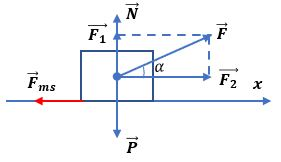
\includegraphics[scale=0.8]{../figs/VN10-PH-30-L-022-1-1.JPG}
			\end{center}
			
			Chọn chiều dương là chiều chuyển động của vật. 
			\begin{equation*}
				F_{\text{ms}} = \mu N=\mu (P-F\sin \alpha) = 3\ \text{N}.
			\end{equation*}
			Áp dụng định luật II Newton theo phương ngang
			\begin{equation*}
				F\cos \alpha - F_{\text{ms}} =ma \Rightarrow a = \text{2,83}\ \text{m/s}^2.
			\end{equation*}
			Quãng đường vật đi được trong 5 giây 
			\begin{equation*}
				s = \dfrac{1}{2}at^2=\text{35,375}\ \text{m}.
			\end{equation*}
			Công của lực F
			\begin{equation*}
				A_{\text{F}} = Fs \cos \alpha =\SI{10}{\newton}\cdot\SI{35.375}{\meter}\cdot\cos\SI{30}{\degree}=\SI{306.4}{\joule}.
			\end{equation*}
			Công của lực ma sát
			\begin{equation*}
				A_{\text{ms}} = F_{\text{ms}}s \cos 180^\circ =\SI{3}{\newton}\cdot\SI{35.375}{\meter}\cdot\cos\SI{180}{\degree}=\SI{-106.1}{\joule}.
			\end{equation*}
			
			\begin{center}
				\textbf{Câu hỏi tương tự}
			\end{center}
			
			Vật 2 kg trượt lên mặt phẳng nghiêng góc $30^\circ$ với vận tốc ban đầu 4 m/s, biết hệ số ma sát trượt là 0,2. Tính công của trọng lực, cho $g=10\ \text{m/s}^2$.
			
			\textbf{Đáp án:} $-\text{11,88}\ \text{J}$.
		}
		\viduii{4}{
			Một người kéo một vật có $m=\SI{8}{\kilogram}$ trượt trên mặt phẳng ngang có hệ số ma sát $\mu=0,2$ bằng một sợi dây có phương hợp một góc $60^\circ$ so với phương nằm ngang. Lực tác dụng lên dây bằng $\vec{F}_\text{k}$, vật trượt không vận tốc đầu với $a=\SI{1}{\meter/\second^2}$. Công của lực kéo trong thời gian 4 giây kể từ khi bắt đầu chuyển động là (lấy $g=\SI{10}{m/s^2}$)
			\begin{mcq}(4)
				\item $\SI{162,5}{\joule}$.
				\item $\SI{140,7}{\joule}$.
				\item $\SI{142,6}{\joule}$.
				\item $\SI{126,7}{\joule}$.
			\end{mcq}
		}
		{\begin{center}
				\textbf{Hướng dẫn giải}
			\end{center}
			
			Quãng đường vật đi được trong 4 giây:
			$$s=\dfrac{1}{2}at^2 = \SI{8}{m}$$
			
			Áp dụng định luật II Newton theo phương thẳng đứng:
			$$F_y + N =P\Rightarrow N = mg -F_y = mg - F \sin \alpha$$
			
			Áp dụng định luật II Newton theo phương ngang:
			\begin{align*}
				F_x - F_\text{ms} &= ma\\
				\Rightarrow\quad F \cos \alpha - F_\text{ms} &= ma\\
				\Rightarrow\quad F \cos \alpha -  \mu (mg - F \sin \alpha) &= ma\\
				\Rightarrow\quad F&=\dfrac{m(a+\mu g)}{\cos\alpha+\mu\sin\alpha}
			\end{align*}
			Thay các giá trị số, ta tìm được độ lớn lực $F$:
			$$F=\SI{35,65}{N}$$
			
			Công của lực kéo:
			$$A=Fs\cos \alpha  = \SI{142.6}{J}$$
			
			\textbf{Đáp án: C}.
			
			\begin{center}
				\textbf{Câu hỏi tương tự}
			\end{center}
			
			Một vật có khối lượng $m=\SI{3}{\kilogram}$ được kéo lên trên mặt phẳng nghiêng một góc $30^\circ$ so với phương ngang bởi một lực không đổi $F=\SI{70}{\newton}$ dọc theo mặt phẳng nghiêng. Biết hệ số ma sát là 0,05, lấy $g=\SI{10}{\meter/\second^2}$. Tổng công của tất cả các lực tác dụng lên vật là $\SI{215}{\joule}$.
			\begin{center}
				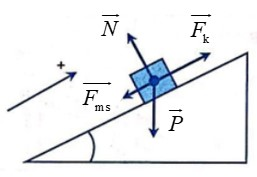
\includegraphics[scale=0.6]{../figs/VN10-PH-30-P-022-1-H2.jpg}
			\end{center}
			Quãng đường tương ứng vật đã di chuyển bằng
			\begin{mcq}(4)
				\item $\SI{1}{\meter}$.
				\item $\SI{2}{\meter}$.
				\item $\SI{4}{\meter}$.
				\item $\SI{6}{\meter}$.
			\end{mcq}
			
			\textbf{Đáp án: C}.
		}
	\end{dang}

\section{Trắc nghiệm}
\begin{enumerate}[label=\bfseries Câu \arabic*:]
	
	\item \mkstar{1}
	
	
	{	Công là đại lượng
		\begin{mcq}
			\item vô hướng, có thể âm hoặc dương. 
			\item vectơ, có thể âm, dương hoặc bằng 0.
			\item vectơ, có thể âm hoặc dương.
			\item vô hướng, có thể âm, dương hoặc bằng 0.
		\end{mcq}
	}
	
	\hideall
	{	\textbf{Đáp án: D.}
		
		Công là đại lượng vô hướng, có thể âm, dương hoặc bằng 0.
	}
	\item \mkstar{1}
	
	
	{	Trường hợp nào sau đây công của lực bằng không?
		\begin{mcq}
			\item Lực vuông góc với phương chuyển động của vật. 
			\item Lực cùng phương với phương chuyển động của vật.
			\item Lực hợp với phương chuyển động một góc lớn hơn $90^\circ$.
			\item Lực hợp với phương chuyển động một góc nhỏ hơn $90^\circ$.
		\end{mcq}
	}
	
	\hideall
	{	\textbf{Đáp án: A.}
		
		Khi lực vuông góc với phương chuyển động của vật thì $\alpha=90^\circ$, khi đó $\cos \alpha =0$, dẫn đến $A=Fs\cos \alpha=0$.
	}

	\item \mkstar{2}
	
	
	{
			Chọn câu \textbf{sai}.
		\begin{mcq}
			\item Công của lực cản âm vì $90^\circ < \alpha < 180^\circ$.
			\item Công của lực phát động dương vì $90^\circ > \alpha > 0^\circ$.
			\item Vật dịch chuyển theo phương nằm ngang thì công của trọng lực bằng $0$.
			\item Vật dịch chuyển trên mặt phẳng nghiêng thì công của trọng lực bằng $0$.
		\end{mcq}
	}
	
	\hideall
	{	
			\textbf{Đáp án: D.}
		
		Vật dịch chuyển trên mặt phẳng nghiêng thì công của trọng lực khác $0$, vì phương của trọng lực không vuông góc với phương của mặt nghiêng.
	}
	
		\item \mkstar{2}
	
	
	{
	Sử dụng một lực $F=\SI{50}{N}$ tạo với phương ngang một góc $\alpha = 60^\circ$ kéo một vật và làm vật chuyển động thẳng đều trên mặt phẳng nằm ngang. Công của lực kéo khi vật di chuyển được một đoạn đường bằng $\SI{6}{m}$ là
	\begin{mcq}(4)
		\item $\SI{0}{J}$. 
		\item $\SI{260}{J}$.
		\item $\SI{300}{J}$.
		\item $\SI{150}{J}$.
	\end{mcq}
	}
	
	\hideall
	{	
		\textbf{Đáp án: D.}
		
		Công của lực kéo:
		$$A=Fs\cos \alpha  =\SI{150}{J}.$$
		
	}
		\item \mkstar{2}
	
	
	{
			Một người kéo một thùng gỗ trượt trên sàn nhà bằng một sợi dây hợp với phương ngang một góc $60^\circ$, lực tác dụng lên dây là $\SI{200}{N}$. Khi thùng gỗ được kéo và trượt một đoạn $\SI{10}{m}$ thì công của lực kéo là
		\begin{mcq}(4)
			\item $\SI{200}{J}$. 
			\item $\SI{1000}{J}$.
			\item $\SI{2000}{J}$.
			\item $\SI{120000}{J}$.
		\end{mcq}
	}
	
	\hideall
	{	
		\textbf{Đáp án: B.}
		
		Công của lực kéo:
		$$A=Fs\cos \alpha = \SI{1000}{J}.$$
	}

		\item \mkstar{2}
	
	
	{
			Vật nào sau đây \textbf{không} có khả năng sinh công?
		\begin{mcq}
			\item Vật đang rơi tự do xuống mặt đất. 
			\item Dòng nước từ trên cao đổ mạnh xuống làm quay tuabin nước.
			\item Vật đang nằm yên trên mặt đất.
			\item Viên đạn đang bay.
		\end{mcq}
	}
	
	\hideall
	{	
			\textbf{Đáp án: C.}
		
		Vật đang nằm yên trên mặt đất không có khả năng sinh công.
	}
		\item \mkstar{2}
	
	
	{Công có thể biểu thị bằng tích của:
		\begin{mcq}
			\item Năng lượng và khoảng thời gian.
			\item Lực, quãng đường đi được và khoảng thời gian.
			\item Lực và quãng đường đi được.
			\item Lực và vận tốc.
		\end{mcq}
	}
	
	\hideall
	{	
		\textbf{Đáp án: C.}
	}
		\item \mkstar{2}
	
	
	{
		Người ta kéo một cái thùng nặng $\SI{20}{kg}$ trượt trên sàn nhà bằng một dây hợp với phương nằm ngang một góc $60^\circ$, lực tác dụng lên dây là $\SI{300}{N}$. Tính công của lực đó khi thùng trượt được $\SI{10}{m}$. 
		\begin{mcq}(4)
			\item $\SI{1000}{J}.$
			\item $\SI{500}{J}.$
			\item $\SI{1500}{J}.$
			\item $\SI{100}{J}.$
		\end{mcq}
	}
	
	\hideall
	{	
		\textbf{Đáp án: C.}
		
		Công của lực $F$ kéo thùng đi được $\SI{10}{m}$ là:
		
		$$A = Fs\cos \alpha = \SI{1500}{J}.$$
	}

		\item \mkstar{2}
	
	
	{Một chiếc ô tô sau khi tắt máy còn đi được $\SI{10}{m}$. Biết ô tô nặng 1,5 tấn, hệ số cản bằng 0,25 (Lấy $g = \SI{9,8}{m/s}^2$). Công của lực cản có giá trị:
		\begin{mcq}(4)
			\item $-\SI{36750}{J}.$
			\item $\SI{36750}{J}.$
			\item $\SI{18375}{J}.$
			\item $-\SI{18375}{J}.$
		\end{mcq}
	}
	
	\hideall
	{	
		\textbf{Đáp án: A.}
		
		Công của lực cản là: 
		
		$$A_\text{cản} = F_\text{ms}s = \mu mgs = \SI{36750}{J}.$$
		
		Vì công cản nên $A < 0 \Rightarrow A = - \SI{36750}{J}.$
	}
			\item \mkstar{2}
	
	
	{Tác dụng lực không đổi $\SI{150}{N}$ theo phương hợp với phương ngang góc $30^\circ$ vào vật khối lượng $\SI{80}{kg}$ làm vật chuyển động được quãng $\SI{20}{m}$. Tính công của lực tác dụng.
		\begin{mcq}(4)
			\item $\SI{2598}{J}.$
			\item $\SI{598}{J}.$
			\item $\SI{298}{J}.$
			\item $\SI{258}{J}.$
		\end{mcq}
	}
	
	\hideall
	{	
		\textbf{Đáp án: A.}
		
		Công của lực tác dụng
		
		$$A=Fs\cos \alpha =\SI{2598}{J}.$$
	}
\end{enumerate}
\hideall
{
	\begin{center}
		\textbf{BẢNG ĐÁP ÁN}
	\end{center}
	\begin{center}
		\begin{tabular}{|m{2.8em}|m{2.8em}|m{2.8em}|m{2.8em}|m{2.8em}|m{2.8em}|m{2.8em}|m{2.8em}|m{2.8em}|m{2.8em}|}
			\hline
			1.D  & 2.A  & 3.D  & 4.D  & 5.B  & 6.C  & 7.C  & 8.C  & 9.A  & 10.A  \\
			\hline

		\end{tabular}
	\end{center}
}
\section{Tự luận}
\begin{enumerate}[label=\bfseries Câu \arabic*:]
		\item \mkstar{2}
	
	
	{
			Một hành khách kéo đều một vali đi trong nhà ga trên sân bay trên quãng đường dài $\SI{150}{m}$ với lực kéo có độ lớn $\SI{40}{N}$ theo hướng hợp với phương ngang một góc $60^\circ$. Hãy xác định công của lực kéo của người này.
	}
	
	\hideall
	{	
		Công của lực kéo của người: $$A=Fs\cos \alpha = \SI{3000}{J}.$$
	}
	
		\item \mkstar{2}
	
	
	{
		Tính công của lực $F=\SI{1200}{N}$ tác dụng lên vật làm vật dịch chuyển quãng đường $\SI{4}{m}$, biết góc hợp bởi chiều của lực và chiều dịch chuyển là $60^\circ$.
	}
	
	\hideall
	{	
		Công của lực: $$A=Fs\cos \alpha = \SI{2400}{J}.$$
	}

		\item \mkstar{2}
	
	
	{
		Con ngựa kéo chiếc xe với một lực kéo $F=\SI{100}{N}$ theo phương nằm ngang. Chiếc xe chuyển động thẳng đều trên đường nằm ngang với vận tốc $\SI{8}{m/s}$ trong thời gian 5 giây. Tính công của lực kéo của con ngựa ở đoạn đường trên. 
	}
	
	\hideall
	{	
		Quãng đường con ngựa kéo xe:
		$$s=vt=\SI{40}{m}.$$
		
		Công của lực kéo:
		$$A=Fs=\SI{4000}{J}.$$
	}
			\item \mkstar{2}
	
	
	{
		Một thùng nước khối lượng $\SI{10}{kg}$ được kéo cho chuyển động thẳng đều lên cao $\SI{5}{m}$ trong thời gian 1 phút 40 giây. Tính công của lực kéo. Lấy $g=\SI{10}{m/s^2}$.
	}
	
	\hideall
	{	
		Lực kéo thùng nước để thùng chuyển động thẳng đều:
		$$F=P=mg=\SI{100}{N}.$$
		
		Công của lực kéo:
		$$A=Fs=\SI{500}{J}.$$
	}
		\item \mkstar{2}
	
	
	{
		Khi rửa gầm xe ô tô, người ta sử dụng máy nâng ô tô lên độ cao $h = \SI{160}{cm}$ so với mặt sàn. Cho biết khối lượng ô tô là $m = \text{1,5}\ \text{tấn}$. Tính công tối thiểu mà máy nâng đã thực hiện.
	}
	
	\hideall
	{	
		Để nâng được ô tô thì máy nâng phải tác dụng vào ô tô một lực có độ lớn tối thiểu bằng trọng lượng của ô tô:
		
		$$F = P =mg = \text{1,5} \cdot 10^4\ \text{N}.$$
		
		Công tối thiểu mà máy nâng đã thực hiện là:
		
		$$A = Ph = \SI{24000}{J} = \SI{24}{kJ}.$$
		
	}
	
	
\end{enumerate}